
%: ----------------------- detector file header -----------------------
\chapter{SNO+ Detector}
\label{sec:detector}

% the code below specifies where the figures are stored
\ifpdf
    \graphicspath{{detector/figures/PNG/}{detector/figures/PDF/}{detector/figures/}}
\else
    \graphicspath{{detector/figures/EPS/}{detector/figures/}}
\fi


% ----------------------------------------------------------------------
% ----------------------- Detector Chapter -----------------------------
% ----------------------------------------------------------------------
% 9385 PMTs comes from doing the following SQL query on DB
%select count(*) from pmt_info where (type & 1)>0 and (type & 32)=0  and (type & 128) =0 and (type & 2)>0 and (type& 64)=0 and (type & 16)=0 and (type & 8)=0;
The SNO+ detector inherits much of its infrastructure from the SNO
experiment~\citep{sno_detector_paper}.
The detector is mostly simply described as a large volume of a
target material that is deep underground and is observed by a large array of
photomultiplier tubes (PMTs).
The target material dictates the physical processes
observable with the detector.
The SNO detector was originally designed for a heavy-water
target, the benefits of a heavy-water target are discussed in Sec~\ref{sec:sno}.
For SNO+ the detector will operate in three separate phases, each with a different
target medium.
For all results in this work the target medium is light-water ($\ce{H_{2}O}$);
this phase is referred to as the ``water phase''.
In the next phase the water is to be replaced by a liquid-scintillator,
LAB-PPO~\citep{mchen_labppo}, that will be the ``pure scintillator phase'' or
just the ``scintillator phase''.
After the scintillator phase the LAB-PPO will be doped with tellurium for
a neutrinoless double-beta decay search, this is referred to as the ``tellurium phase''.
The motivations for each phase is discussed in Ref.~\citep{snop_status_prospects}.

\begin{figure}[htbp]
\centering
\begin{subfigure}[b]{0.3\textwidth}
\centering
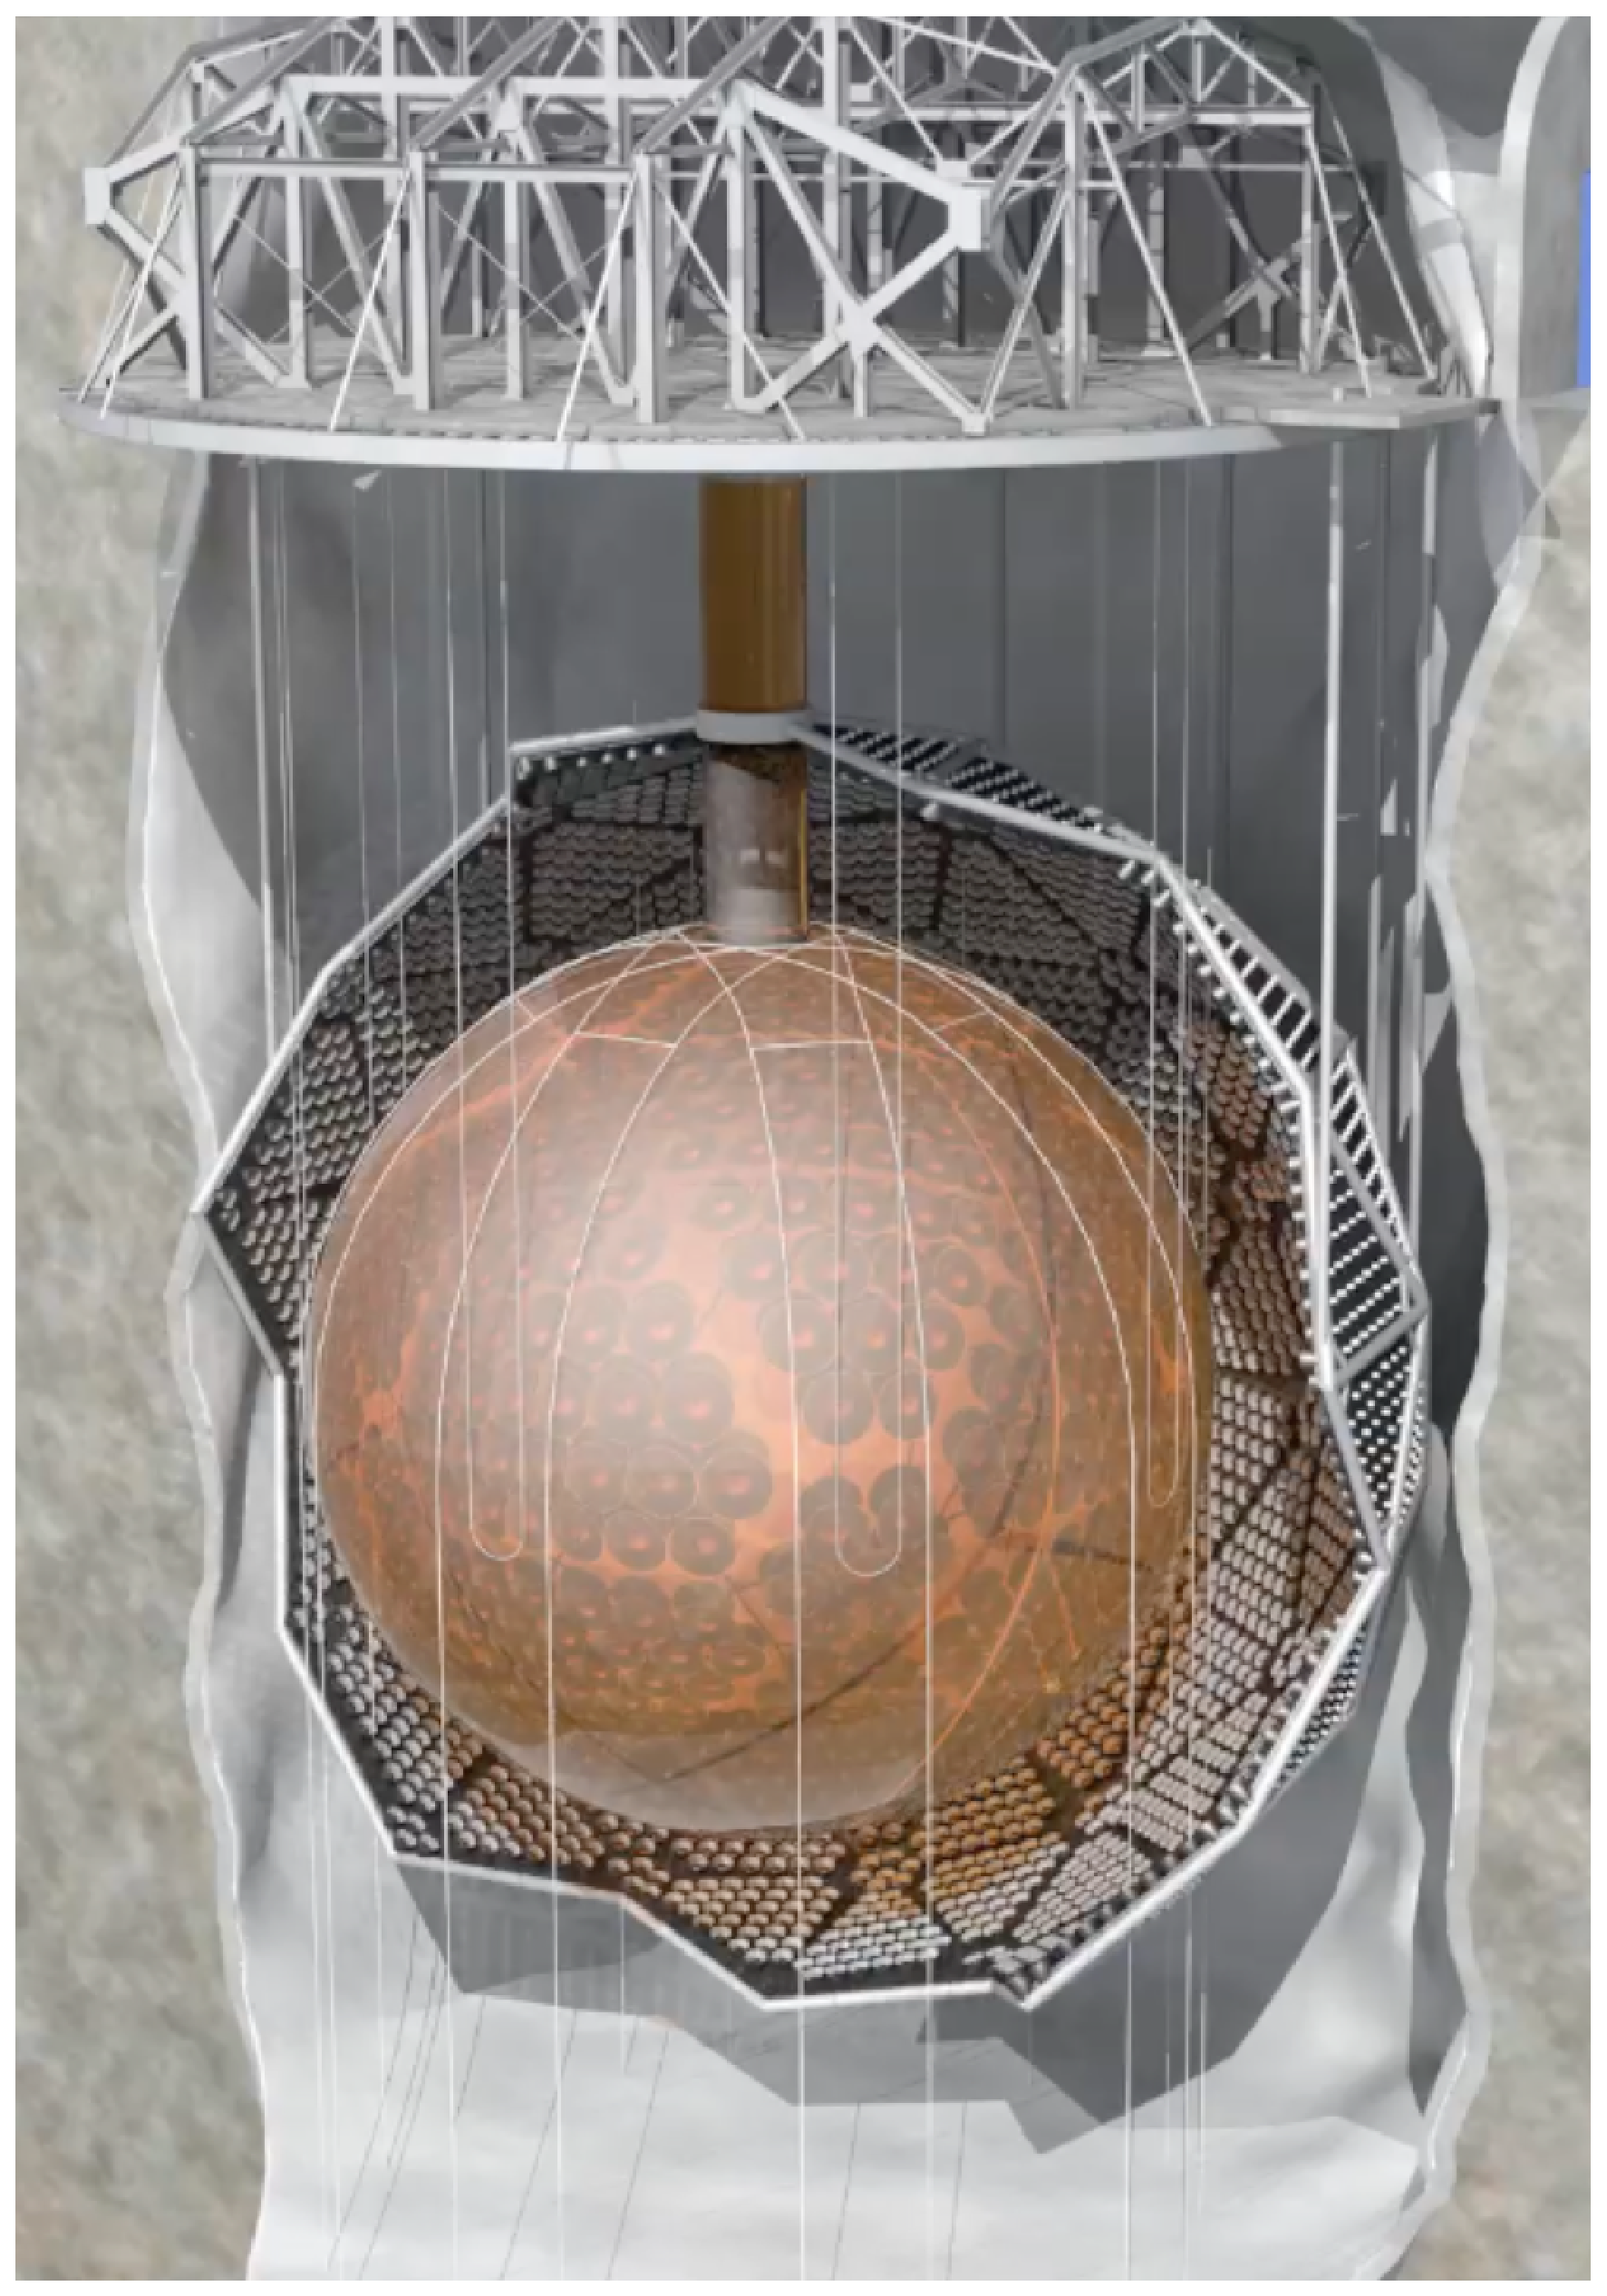
\includegraphics[width=1\textwidth]{cavity}
\caption[SNO+ Diagram] {}
\label{fig:snop_diagram}
\end{subfigure}

\begin{subfigure}[b]{0.6\textwidth}
\centering
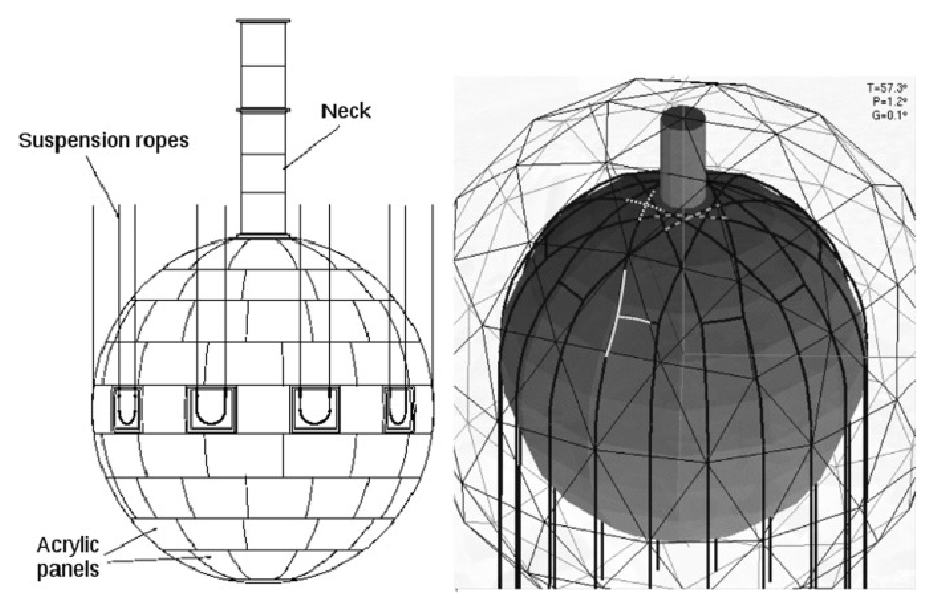
\includegraphics[width=1\textwidth]{rope_net}
\caption[SNO+ Ropes]{}
\label{fig:ropes}
\end{subfigure}

\label{fig:snop_diagrams}
    \caption[SNO+ Detector]{(a) Drawing of the SNO+ showing the
    AV, PSUP, cavity, neck, ropes, and upper deck. (b) Schematic
    depiction of the AV and hold-up and hold down ropes.}
\end{figure}

The detector's target volume is encapsulated within a 6-meter radius spherical acrylic vessel (AV),
which is held suspended in a large cavity filled with ultra-pure water (UPW)\@.
The acrylic sphere has a 6.8\,m acrylic chimney, called the ``neck'', at its top
to allow access to the detector volume.
Surrounding the acrylic vessel is an  array of inward pointing PMTs.
The structure holding these PMTs is referred to as the PMT Support Structure
(PSUP).
Figure~\ref{fig:snop_diagram} depicts the SNO+ detector.

There are roughly 90 PMTs on the PSUP that point outward, towards the surrounding cavity
walls.
These outward looking tubes are called OWLs and are for the purpose of tagging
particle interactions that occur outside the PSUP\@.
There are an additional three tubes mounted at the top of the neck of the AV,
these are referred to as NECK tubes.

%, which have typical quantum efficiency of  $XXX$\%.

\begin{figure}[htbp]
    \centering
    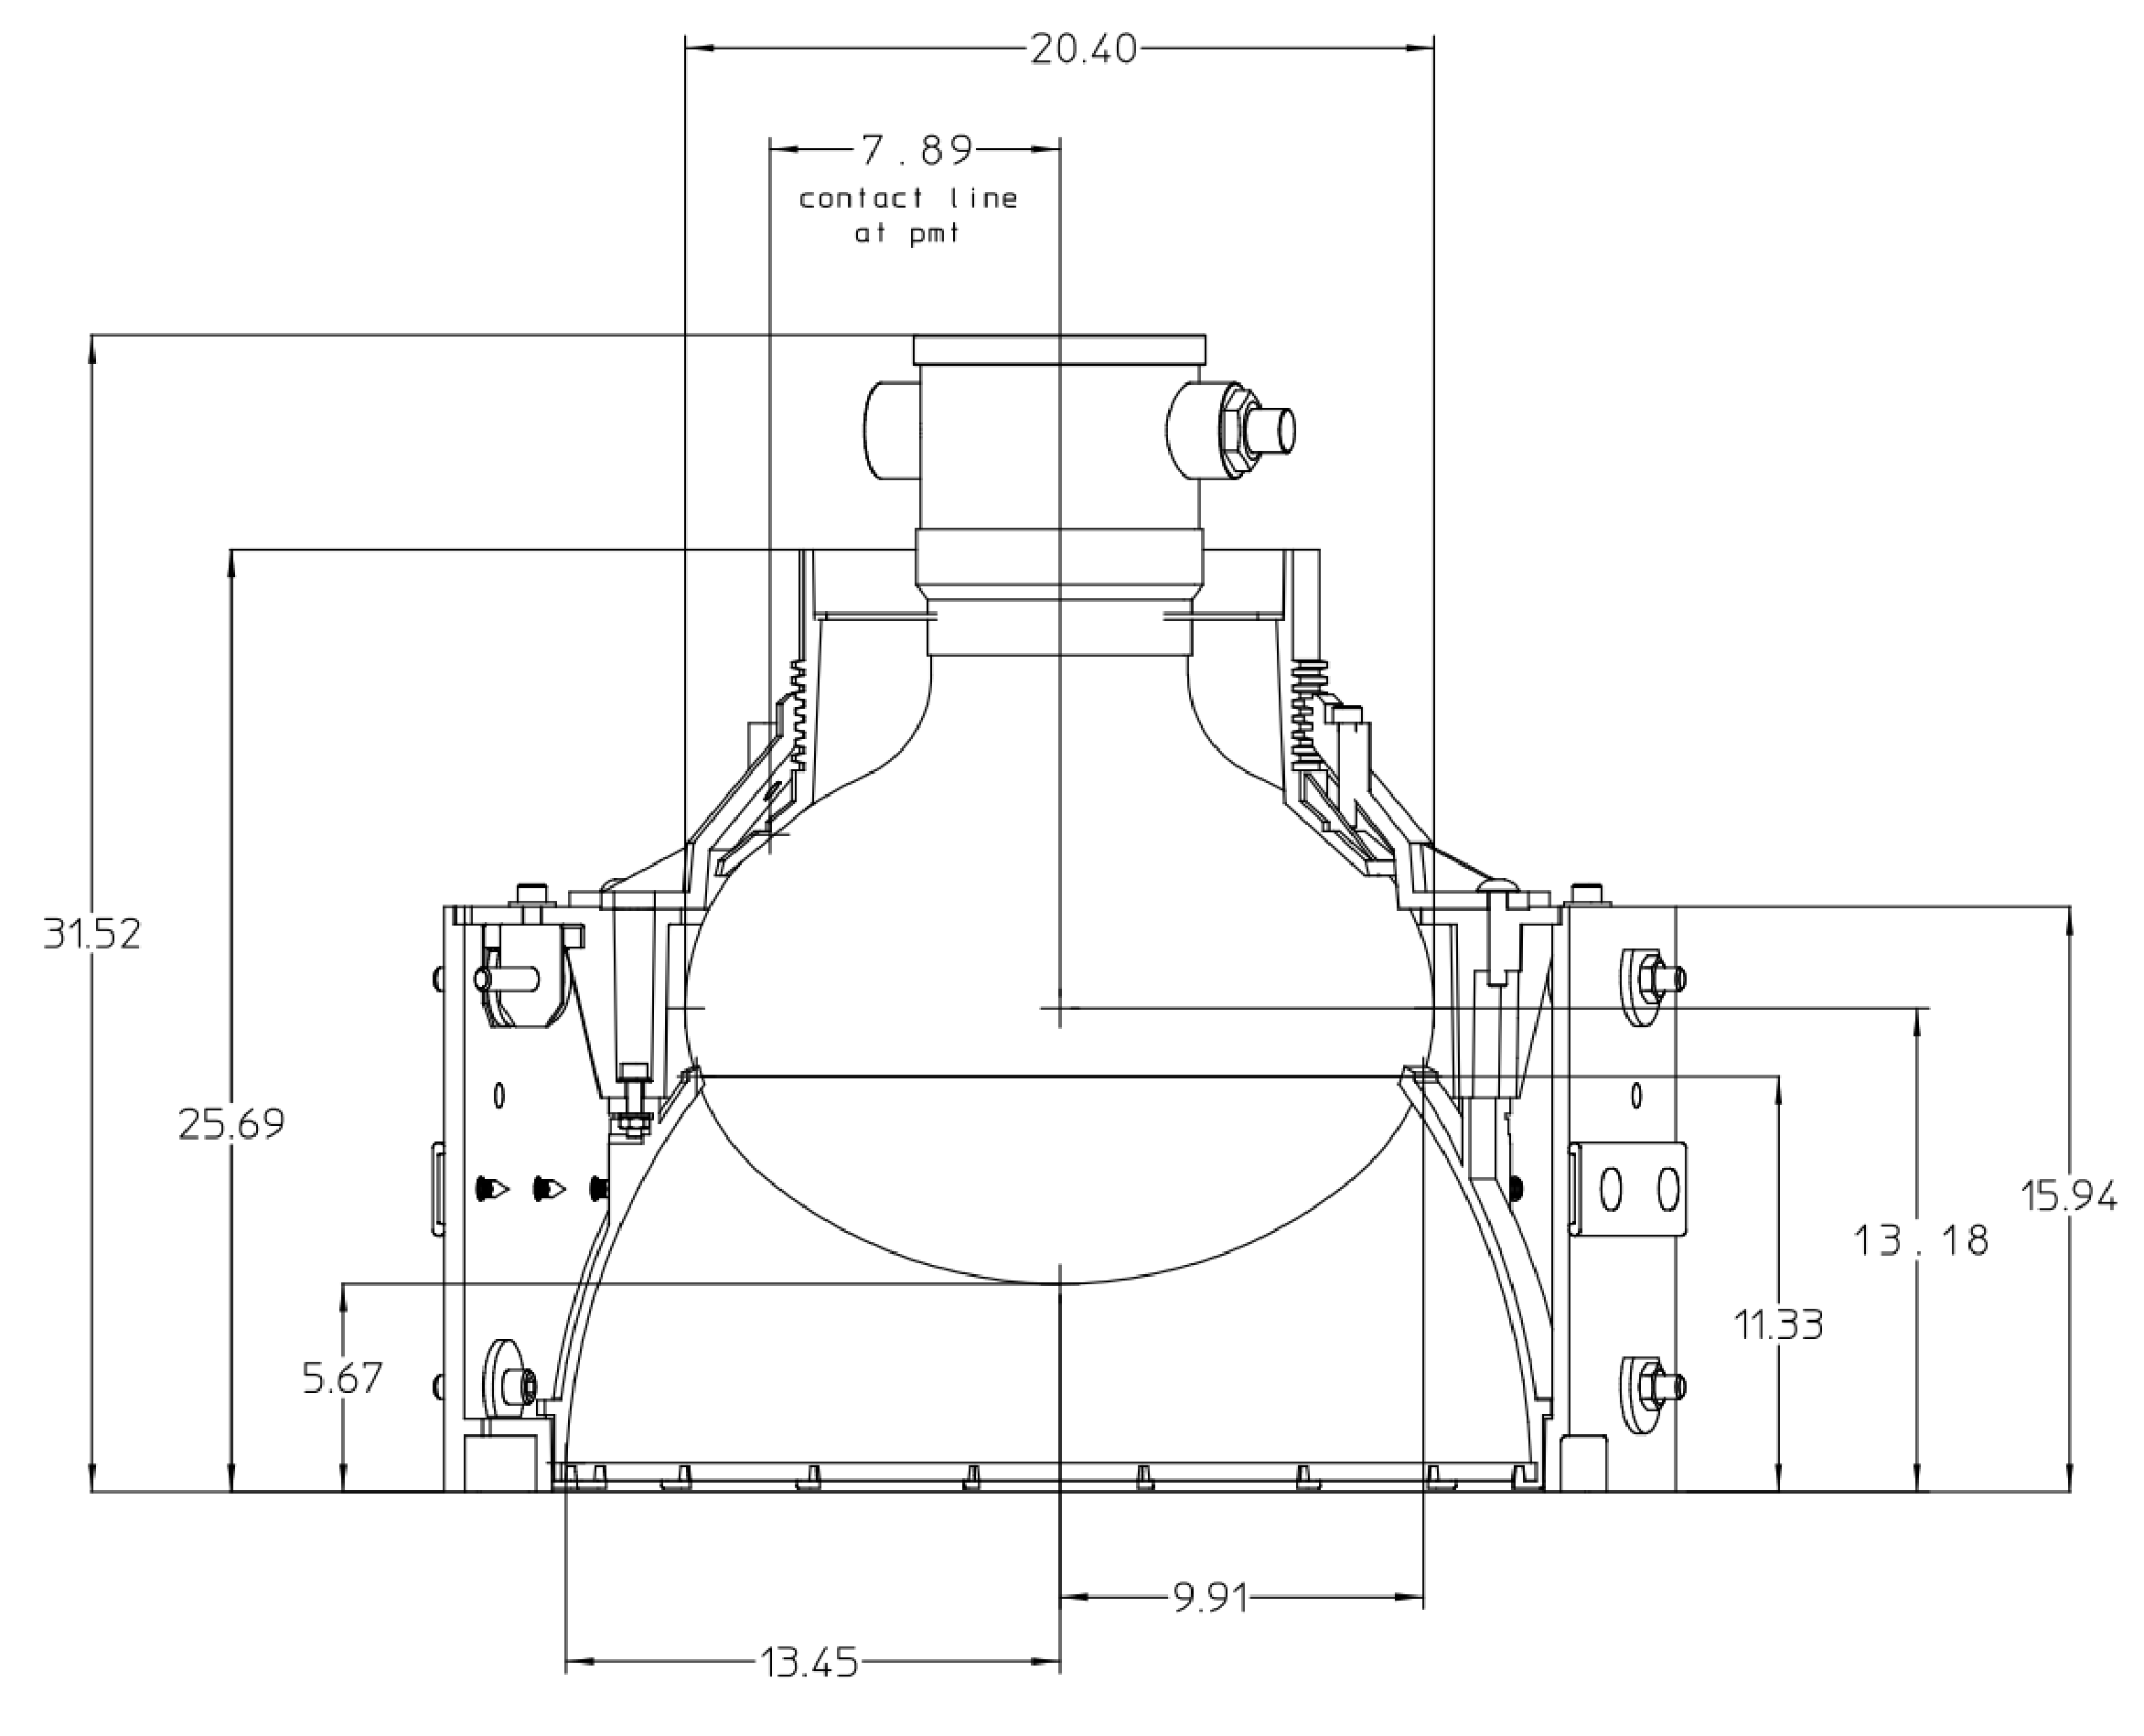
\includegraphics[width=0.7\textwidth]{sno_casette}
    \caption[PMT Casette] {Schematic diagram of the SNO/SNO+ PMT and
    PMT housing. Dimensions in cm. Figure from~\citep{sno_detector_paper}.}
\label{fig:sno_pmt_casette}
\end{figure}

SNO+ has 9385 inward looking PMTs all mounted in the PSUP at an average radius
of 8.4\,m from the center of the detector..
All PMTs are Hammatsu R1408 8-inch PMTs.
The inward looking PMTs are all housed within a plastic cassette,
and each PMT is also surrounded by an array of reflective
petals arranged in a Winston cone~\cite{winston}.
The reflective petals serve to increase the effective photo-sensitive area
of the PMT and are typically referred to as the PMT ``concentrator''.
With the concentrators the approximate geometric coverage of the PMT array is $55\%$,
accounting for the angular acceptance and reflectivity of the concentrators gives
an effective coverage of approximately $50\%$.
Figure~\ref{fig:sno_pmt_casette} shows a schematic diagram of the PMT and
its housing.

For the scintillator and tellurium-loaded phases the AV volume will have
a lower density than the surrounding water volume, resulting in significant buoyant
forces on the AV\@.
To counteract the buoyancy a hold-down rope-net was installed across the top
of the AV, and anchored to the cavity floor.
A number of PMTs were removed from the PSUP to allow the rope to pass through.
Figure~\ref{fig:ropes} depicts the rope-net.

Above the cavity volume is an optically isolated deck on which all the detector
readout and trigger electronics are kept.
The PMT housing provides a BNC-like connection that allows the 2kV power 
supply to be provided to each PMT and allows for the PMT signals to be read
out.

\section{Detection Mechanism}
The goal of the SNO+ detector is to detect and record information about as
many of the photons produced within the AV as possible.
By observing photons information about the physical processes that produced
the light can be inferred.
Cherenkov radiation is the primary photon generating process of interest in
SNO+'s water-phase.
Cherenkov radiation is produced by any charged particle moving with
velocity ($\vec{v}$) such that $\abs{\vec{v}} > \frac{c}{n}$, where $c$ is the speed
of light and $n$ is the index of refraction in the target medium~\citep{cherenkov}.

The produced Cherenkov light has a few properties that make it a desirable
method for particle detection.
The first is that the number of photons produced scales nearly linearly
with the energy of the particle propagating, therefore the energy of the particle
can be estimated by simply counting the number of detected photons.
The second desirable property is that the produced photons will be
emitted in a cone, with an opening angle of approximately $42^{\circ}$ with
respect to the particle's direction of travel.
Meaning by detecting Cherenkov light the particles direction of travel
can be inferred.
And finally, if the time of each detected photon is well known then
the requirement that all photons travel from the same point at the same speed
allows the position of the particle to be deduced.
SNO+ takes advantage of each of these aspects of Cherenkov radiation to reconstruct
the position, time, energy, and direction of all interacting particles in the
detector.
The methods used for deducing each value is detailed in Sec~\ref{sec:reconstruction}.

For the scintillator and tellurium-loaded phases scintillation processes will be
the dominant photon production mechanism.
The Cherenkov light production is approximately the same in scintillator as it is in
water, however the ratio of light produced by scintillation processes to Cherenkov
light is approximately 100:1.
With SNO+ it's not expected to be possible to infer which detected photons are
from scintillation processes and which are Cherenkov radiation, so it can be treated
as though all light is from scintillation.
Many people are developing methods to separate Cherenkov light from scintillation
light~\citep{tanners_paper,javi_chess, winslow_directionality},
and so this may be possible for SNO+ in the future.

The primary neutrino interaction that SNO+ is sensitive to is elastic scattering (ES)
off electrons,
Charged and neutral-current nuclear interactions occur as well with the oxygen in the water,
however these are rare and cannot be uniquely to identified against radioactive
backgrounds, and so are ignored.
The cross-section for the ES interaction is discussed in~\ref{sec:esxsec}.
The forward peaked angular cross-section means that information about the
neutrino direction is maintained in the interaction.
But the differential cross-section for recoil energy is nearly flat below the
end point. Meaning relatively little information about the incoming neutrino energy
is preserved by the interaction.

%For the SNO+ water-phase the scattered electron generates light via Cherenkov radiation,
%assuming it's above Cherenkov threshold for water which is $XXX$\,MeV.
%If it is above the Cherenkov threshold the electron will generate photons that
%travel at approximately a 42$^{\circ}$ angle to the direction of the electron.
%The angle of travel comes directly from the speed at which electro-magnetic
%signals propagate in the medium.
%Figure $TODO$ shows this diagrammatically, as the charged particle (in this case
%an electron) distance $\ell$ from point A, to point B, the electro-magnetic wave
%that was emitted at A will travel a distance $\ell \dfrac{c}{v}$, forming
%a spherical wavefront at that distance.
%When the electron travels another distance $\ell$ from B to C the wavefront
%from A is a distance $2\ell\dfrac{c}{v}$ from A and the wavefront from B is
%a distance $\ell \dfrac{c}{v}$ from B.


%The photons can the be detected by the SNO+ PMT array, and the pattern
%of hits analyzed to determine the electron direction, energy, and position.



\subsection{Electronics And DAQ}
The hardware the connects to and reads out the PMT array forms the SNO+ data acquisition (DAQ)
system\@.
The SNO+ data acquisition (DAQ) inherits much of its design and components from
SNO\@.
There are a few notable upgrades that were made for the purpose of handling the
higher light yield and event rate that SNO+ has compared to SNO\@.
The DAQ hardware can be described as a few separate systems, the trigger system,
the readout system, and the PMT interface system.
The PMT interface provides an approximately 2\,kV (HV) supply to each PMT and provides
the signal from the PMT to the rest of the DAQ electronics.
The trigger system's purpose is to decide when an interesting interaction
within the detector has occurred, and to start the readout process when such an
interaction has occurred.
The readout process is responsible for ensuring enough information about each
PMT signal is recorded such that offline analysis is possible.

The first step of the PMT interface system is the PMT base. The base is responsible
for fanning-out the supplied HV to the PMT dynode pins and connecting the PMT output
to a PMT cable. The PMT base is housed within a water-tight cassette.
The PMT cables pass through penetrations in the cavity ceiling where they then connect
to the rest of the electronics. The PMT cable connects first to a PMT interface
board (PMTIC). The physical connection occurs on a daughter card, called a ``paddle card'',
that accommodates up to eight PMT cables; Each PMTIC hosts four paddle cards.
The PMTIC is responsible for fanning out the PMT high voltage
to each PMT and providing channel level adjustment to the voltage
each PMT receives; the voltage adjustment is done with a series of
swappable resistors.
The PMTIC is also responsible for separating the PMT signal from the supplied
HV, this is achieved with a capacitative decoupling circuit.
Once the two signals are separated the PMTIC sends the PMT signal to
a front end card (FEC) via a board-to-board connector, where it enters
the readout and trigger system.

That signal is compared to a threshold, if the signal is over threshold a ``hit''
has occurred --- this threshold is often called the ``channel threshold''.
At the time of the channel threshold crossing the following processes occur, the name for each is given
in parenthesis:
a 100\,ns long fixed-height square pulse is created (N100), a 20\,ns fixed height square pulse is created (N20),
a high gain copy of the signal is created (ESUMH), a low gain copy of the signal
is created (ESUML), a linear voltage ramp begins (TAC ramp), the signal is integrated for
50\,ns with high gain (QHS), the signal is integrated for up to 400\,ns with high gain (QHL),
and the signal is integrated for 50\,ns with a low gain (QLX).
These signals and values are created on a few different custom ASICs on the
daughter boards.
The trigger system uses the first of those 4 signals (N100, N20, ESUMH, and ESUML).
The readout system uses the latter four values (TAC, QHS, QHL, QLX).

The trigger signals are all combined with their counterparts from
other PMT channels across the detector, \textit{i.e.} the N100 signals
from all channels with be combined and separately all the
N20 signals will be combined, \textit{etc}.
The signals are combined through analog summation, summing is done on a few different
circuit boards within the detector.
The FEC sums its top and bottom sixteen channels separately, the crate
trigger card (CTC) sums the signals from the sixteen
FECs that are in each electronics crate.
The signals from each of the nineteen CTCs are all summed on the
Master Trigger Card - Analog (MTCA+). The SNO+ MTCA+ is an upgraded
version of the SNO MTCA\@; more information about the MTCA+ is available in
Sec.\,\ref{sec:mtcap}.

Separate, but identical, MTCA+s are used for each of the four trigger signals.
Each MTCA+ performs the analog summation with three different gains,
resulting in a total of twelve signals spread across four different boards.
Each of the twelve signals are separately compared to a threshold;
each of the twelve thresholds are independent from each other.
These thresholds are called ``trigger thresholds''.

The different gains are in place due to the practical difficulty of maintaining
a good signal-to-noise ratio (SNR) without limiting the range of the
system.
For example, if there exists 10\,mV of noise in the system a 20\,mV pulse
would give a 2:1 SNR, however this would mean if 5000 PMT hits occurred simultaneously
the signal would be 100\,V in size.
It is not practical to have a system with 100\,V range and 20\,mV resolution,
so the three different gain paths allow for three different trade-offs between
SNR/resolution and range.
The highest gain signal has the best SNR, but the smallest range, and so usually
the highest gain signal has the lowest effective threshold.
The reason being that it's more important to have single hit resolution at a threshold
of 8-hits than it is at a threshold 25 hits.
The different gains on each signal are therefore labelled by their threshold (not their gain), e.g.
the high, medium and low gain paths for the N100 signal are respectively called
N100 Low (N100L), N100 Medium (N100M), and N100 High (N100H).

Although there are twelve signal-gain combinations available only seven are
used: N100-Low, N100-Med., N100-High, N20-Low, N20-Med (also called just N20), ESUMH-Low, and ESUML-Low.
Since the ESUMH and ESUML each only use one gain path, they're usually
referred to simply as ESUMH and ESUML with their gain path understood to be
the high gain path.

When a trigger signal goes over its threshold a 20\,ns digital pulse is
emitted for that signal. This pulse is called a ``raw-trigger'' and there is
one for each of the seven used trigger signals.
The raw-trigger signals are sent from the MTCA+s to the Master Trigger
Card-Digital (MTCD).
Finally, each of these seven raw-trigger signals can be masked in or masked out on
the MTCD\@;
if a raw-trigger is masked out, nothing happens when it fires,
if it is masked in, then the raw trigger creates a ``global-trigger'' (GT) signal.
That global trigger signal is fanned out to all the data crates which
in turn sends the GT to all front end cards and daughter boards.
As the GT signal is created the MTCD also generates a signal
called Lockout (LO). Lockout is typically a 420\,ns long pulse and while
the signal is high the MTCD will not create any more global triggers.

Once the global trigger is created the trigger cycle is complete and
the readout process begins.
The raw-trigger signal that caused the global trigger, as well as any other
raw-trigger signals that were high within a 20\,ns window of the global trigger,
are recorded and readout, this is know as the ``trigger word''.
When the GT is created a counter, called the global trigger identifier (GTID) is incremented
and readout along with the trigger word.

The four values that are created by the PMT signal crossing
the channel threshold (TAC, QHS, QHL, QLX) are stored in analog memory
cells on the daughter boards.
They are stored for a length of time known as ``GT\_VALID'', if
a GT does not arrive before GT\_VALID expires the TAC, QHS, QHL, \& QLX values
are discarded. A typical value for GT\_VALID is $400\,ns$, although
there exists some channel\,-\,to\,-\,channel variation.
If a GT signal does arrive at the channel before GT\_VALID expires the
values in the memory cells are digitized and readout to a memory buffer
on the FEC\@.
The TAC ramp starts when the PMT signal crosses channel threshold
and stops when the GT signal arrives at the channel.
Since the TAC voltage ramp is linear over time the value of the TAC
indicates when the hit occurred relative to the GT signal.

The FEC stores those values and adds information to identify which
channel's data is stored, it also records the value of its own GTID\@.
Each FEC keeps a counter that is incremented every time it receives a global
trigger signal, in principle the value of this counter will always be the same
as the MTCD GTID, and the same as the counter in every other FEC in the detector.
The GTID counter is our only way of associating recorded hit data with each other
and with the trigger word.

In practice it's possible for a channel's GTID to become out of sync with the GTIDs of
all other channels.
This can result in the hits on a particular channel being associated with
the wrong event.
To mitigate this problem every $2^{16}$th and $2^{24}$th GT respectively creates a $SYNC$ and
$SYNC24$ signal, those signals are sent by the MTCD to each FEC \& DB\@.
If a FEC or DB receives either of these synchronization pulses but its own GTID counter is not
at an increment of $2^{16}$ or $2^{24}$ then the channel is identified as out of sync.
If this happens, the GTID counter is adjusted to the correct value and the next hit to read out from the out of sync channel/channels is accompanied
by a flag to indicate that it was out of sync.
This system ensures a channel is never out of sync for more than $65536$ events.

A short while after the data and the associated identifying information and status flags are buffered
in FEC memory, the data is readout by a create level readout card,
the ``XL3''.
The XL3 is new to SNO+; it replaces the XL1 and XL2 from SNO, more will be said about the
XL3 in Sec.\,\ref{sec:xl3}.

Each data crate has its own XL3, all XL3s read out and serve data asynchronously.
The data-server process receives data from each XL3 and relays that data to
any clients that have subscribed to the PMT data feed.
A similar process is done for the trigger word data. The MTCD sends trigger data
to the data-server, the data-server relays that data to any clients that have subscribed
clients.

The primary client to the data server is what's known as the ``Event Builder'', sometimes
called the EB or just the ``Builder''. The Builder receives data from the data-server and
uses GTID information to associate trigger words and hits with each other.
Once all the hits for an event have been associated with their trigger word the event
has been ``built'' it is written to disk and the read out process for that event is complete.
Data is typically taken in hour long chunks referred to as a ``run'';
every run has an unique number associated with it and a ``run type'' number that
gives basic context to the detector circumstances and settings in which the data was taken.
The Builder, in addition to building events, is responsible for associating
events with their run number and run type.

There are a few ancillary systems within the DAQ electronics, all
of which are new to SNO+.
The first is the CAEN v1720, commonly
referred to as just ``CAEN'', which is a 12-bit digitizer board.
It's role follows from the Analog Measurement Board (AMB) used in
SNO.
The CAEN is used to digitize and readout the trigger signals.
It has eight available input channels that it can digitize, however,
typically only three signals are actually used, those channels digitize ESUMH, N20L, and
N100L. The CAEN's digitization window and sampling rate can be varied,
most commonly the digitization window is 420\,ns and the sample width
is 4\,ns. The CAEN receives a copy of the global trigger allowing and
it keeps it's own GTID counter so its data can later be associated
with the appropriate hit and trigger data. It also receives a copy of the
SYNC and SYNC24 signal so it's synchronization can be ensured.

The input voltage range for the CAEN is an adjustable 2\,V window.
The voltage range for the trigger signals is 10\,V.
The difference in ranges necessitates some way of reducing the range of the trigger signals
before they're sent to the CAEN\@.
The simplest way of reducing the voltage range is to use a voltage
divider to attenuate the signal by a factor of five.
Attenuation has a few undesirable effects though.
The full range of the trigger signal is 10\,V, but the vast
majority of events will only use a small fraction of that range.
So for events that use a small amount of the available 10\,V a factor
of five attenuation will make the signal much smaller than it needs to be,
resulting in loss of information because the signal will be smaller than
the analog noise, or from the noise digitization process itself.
And for the purpose of most analyses that use the data from the CAEN
it's more important to be able to resolve a single hit than to resolve
the height of the full pulse if the pulse is very large.

A scheme for fitting the trigger signal into the CAEN's available range that
optionally allows for either single hit resolution or preserving the full
signal range was adopted.
The trigger signal is clipped within the first 2\,V, thereby retaining full
resolution for small signals, but losing resolution for signals that go over
2\,V.
A board was designed to optionally clip or attenuate the trigger signals
before digitization, for the vast majority of the data taking the signals
were clipped.
I designed the board that performs this analog signal processing,
it's discussed in further in~\ref{sec:tubii}.

%The board that was designed, in part, for this purpose is the Trigger Utility
%Board Mark\,-\,II (TUBii).
%Beyond modifying the trigger signals for the CAEN TUBii plays a significant
%role as part of the trigger and data readout systems as well.
%It's significance comes primarily from the fact that it acts as an auxiliary
%digital trigger board. It can receive raw-trigger pulses from the MTCA+s and apply
%customizable trigger logic to them and emit it's own raw-trigger pulses which are
%sent to the MTCD\@.
%TUBii also receives the global trigger signal and produces its own trigger
%word based upon which raw trigger pulses it had received. The TUBii trigger
%word is synchronized with the rest of the data for each event through it's own
%global trigger counter and through the SYNC/SYNC24 signals. More information about
%TUBii's role in the DAQ can be found in Sec.~\ref{sec:tubii}


\section{Electronics Upgrades}
\label{sec:upgrades}
As previously mentioned, in SNO+'s scintillator and tellurium-loaded phases the
amount of light produced by any interaction is expected to be roughly a factor
of $100$ greater than the light that would be produced by a water target.
This increase in photon production translates to an equivalent increase in the
current in the trigger system and the necessary data read out rate.
Between the time when the original SNO DAQ electronics was designed and now,
the availability and sophistication of commercial computing and DAQ hardware
has increased dramatically.
To accommodate the increased current and data volume and to take advantage of modern
hardware a few key pieces of the SNO DAQ was upgraded as part of the change from
SNO to SNO+.

Beyond the need to increase the improve the DAQ for the higher expected light
yield there were a few aspects of the SNO electronics that motivated several
features in the upgraded electronics.
Most notable of these is the unstable analog trigger baseline.
The voltage of any trigger signal's baseline can vary.
The baseline of the each trigger signal is the voltage observed
when there are zero hits in the analog sum,
As the baseline moves closer to or further from the trigger threshold
the number of PMT hits required to trigger the detector changes.
The result is a difficult to understand trigger efficiency and bursts in the trigger
rate that can overwhelm the DAQ\@.

The baselines are sensitive to a number of known factors such as the
ambient temperature, the PMT noise environment, and settings
on the front-end.
There are also a number of factors that effect that are more difficult
to identify, such as transistors on the CTC performing malfunctioning due to
age or other unknown factors.
These factors lead to the baseline for any trigger signal varying
by up to a few hits over the course of a few hours.
A common source of baseline variation is known as ``dropout'';
dropout is single nhit shifts in the  baseline that persist over an indefinite
time period with no clear signature in the readout.
Dropout will be discussed in detail in~\ref{sec:dropout}.

\subsection{XL3}
\label{sec:xl3}
The SNO DAQ used a centralized serial readout system, where each crate of
electronics was read out in one after the other.
As part of the electronics upgrade from SNO to SNO+ this system was changed to
an asynchronous, parallel readout system, allowing for a significant increase in
the data readout speed.
The board responsible for this is the XL3 which hosts a Xilinx ML403
Evaluation platform.
The ML403 uses a Xilinx Vertex-4 FPGA as its primary logic chip and has
64-MB of supporting SDRAM and persistent memory provided by a CompactFlash
card.
The XL3 \& ML403 interface with the FECs in a crate through VME-like communication
across the ``SNOBUS'' backplane.

\begin{figure}[htbp]
    \centering
    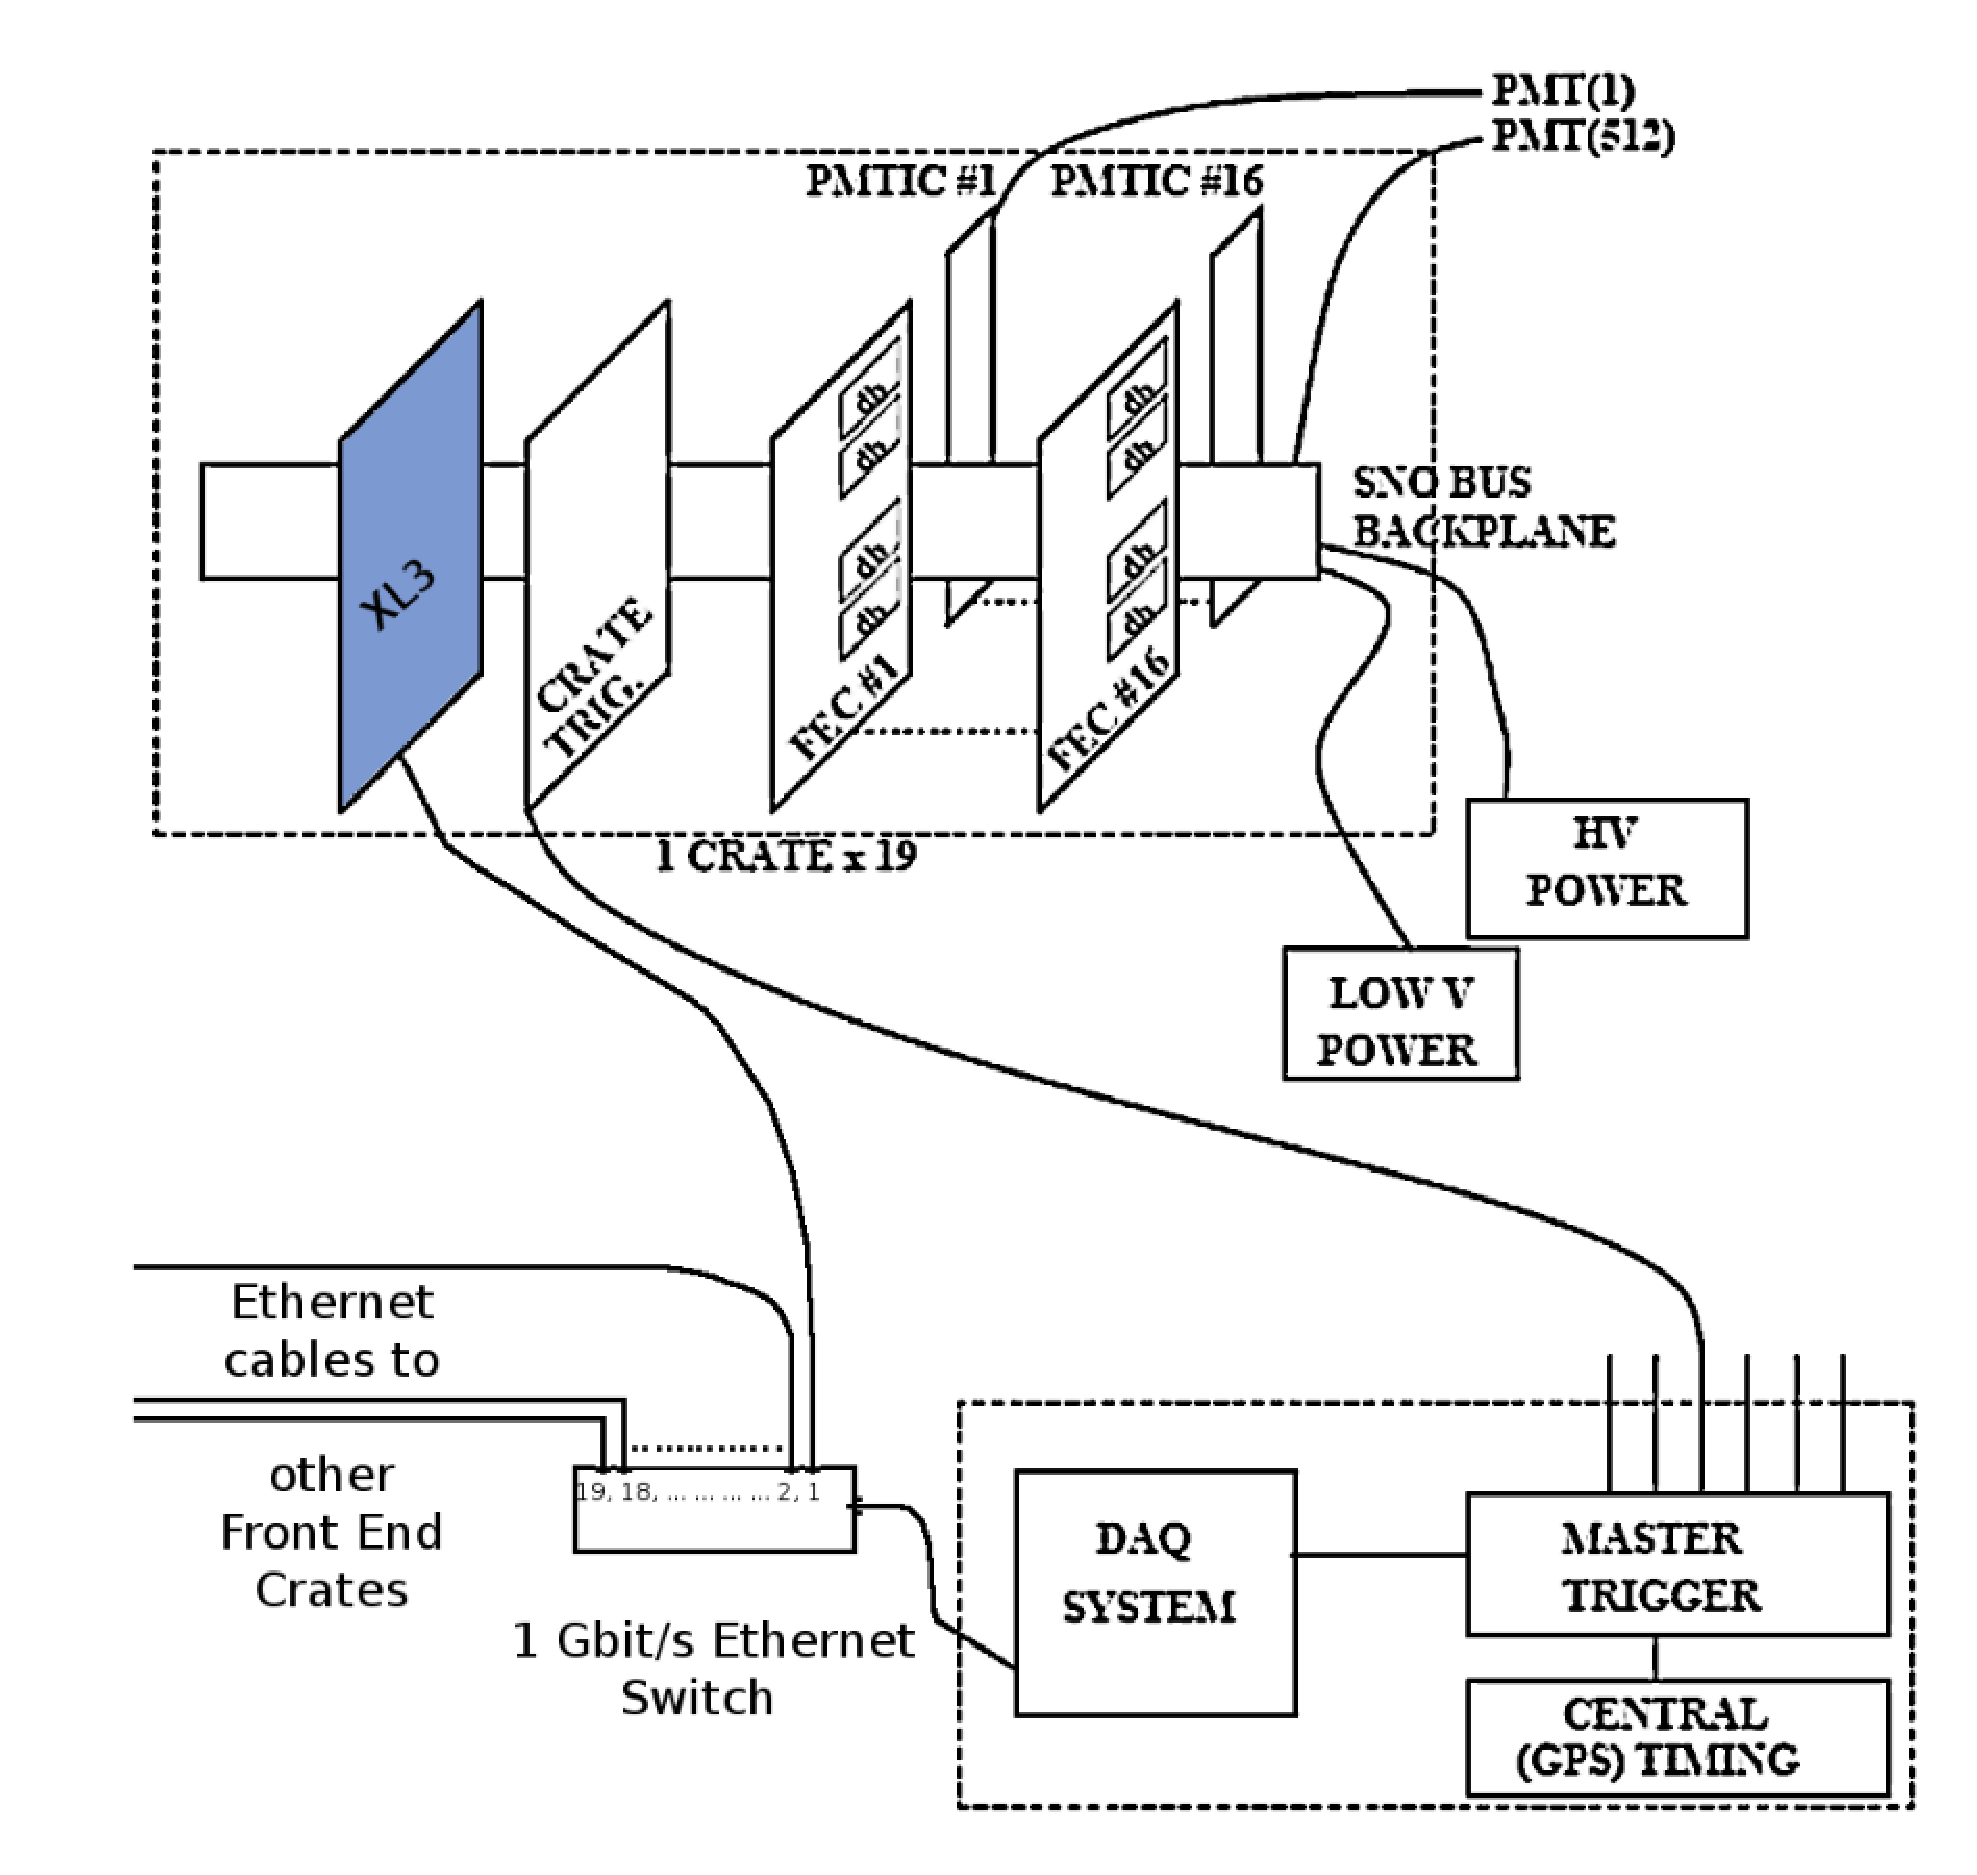
\includegraphics[width=0.5\textwidth]{xl3_daq_diagram}
    \caption[SNO+ DAQ Diagram]{Diagram of the SNO+ DAQ\@.
    Figure from~\citep{richie_thesis}.}
\label{fig:xl3_daq_diagram}
\end{figure}

The XL3 reads data from the FECs across the backplane, and buffers that data
in on-board memory before reading it out to a central DAQ computer over Ethernet.
The maximum data rate each XL3 is capable of is approximately
14\,MB/s, yielding a detector-wide rate of 250\,MB/s.
This translates to being able to read out out roughly one-hundred thousand
hits per crate per second.
Figure~\ref{fig:xl3_daq_diagram} shows schematically how the XL3 is
incorporated into the SNO+ DAQ\@.

\subsection{MTCA+}
\label{sec:mtcap}
\begin{figure}[htbp]
    \centering
    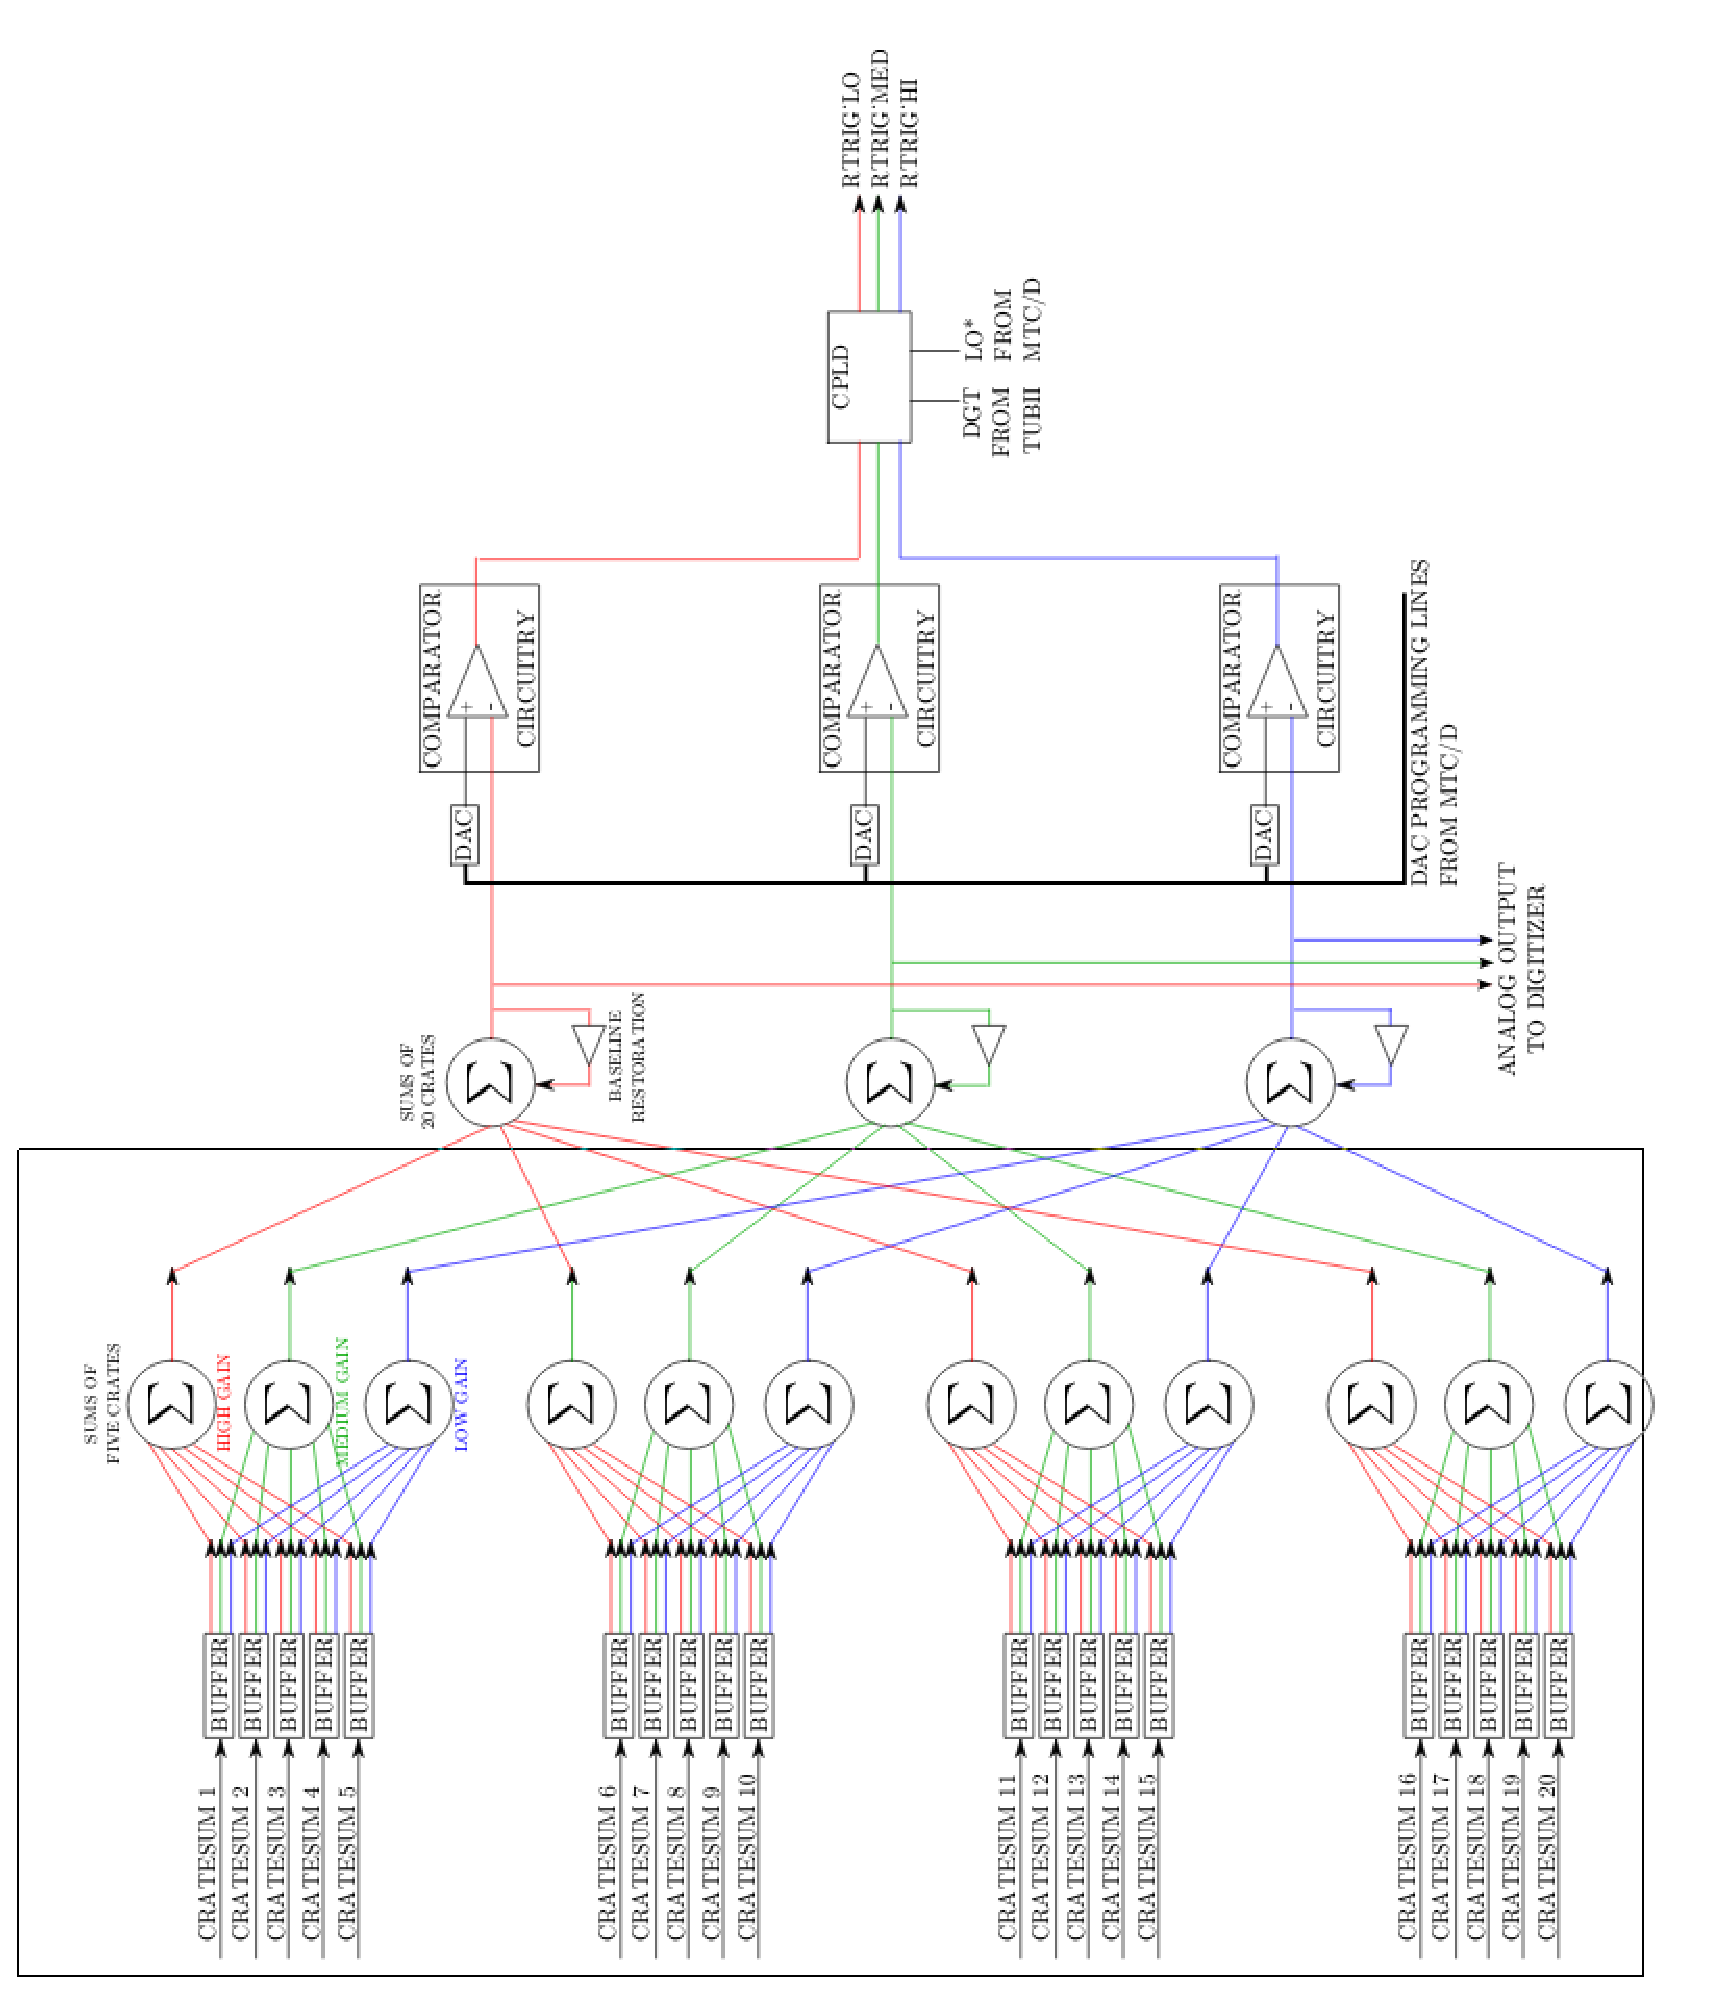
\includegraphics[width=1\textwidth]{mtcap_analog_diagram}
    \caption[MTCA+ Analog Diagram]{Schematic diagram of analog
    summation in the SNO+ trigger system. Figure courtesy of
    Andy Mastbaum.}%TODO cite Andy's thesis maybe? Or the MTCA+ user guide?
\label{fig:mtcap_analog_diagram}
\end{figure}

The SNO MTCA was not expected to be able to operate at the expected
hit rate and occupancy of SNO+ in its scintillator or tellurium-loaded phases.
So the primary goal for the MTCA+ is to simply replace the analog summing
and discriminating capabilities of the SNO MTCA, and perform stably
at the higher rates expected in SNO+.
For this reason the MTCA+ performs the analog multiplicity sum using a series
of high-current voltage feedback operational amplifiers.
%The gain of the three different analog is 1:1, 1:3.6 and 1:10. XXX include this?

One of the most transformative changes that the MTCA+ introduces into
the SNO+ trigger system is its baseline restoration circuitry.
In SNO typical baseline variations could be tolerated because
the threshold was far from the baseline, so variations of a few hits
did not typically have a very large effect.
In SNO+, due to many of the upgrades, a significantly lower threshold was achieved,
so a variation a few hits causes a much larger change in the trigger rate,
leading to a higher likelihood of triggering faster than the  maximum possible
readout rate.

The MTCA+ provides two ways to mitigate baseline variations.
The first is that the MTCA+ provides a relay to dynamically enable or disable each
crate's participation in the trigger sum.
This is useful if a CTC fails, its trigger sums can be disabled to prevent it from
pulling up/down the entire trigger sum to the point that stable triggering is no
longer possible.
This situation is rare, but the ability to disable individual
crates in those situations is useful for diagnosing and isolating issues.

The second is baseline restoration circuit on the MTCA+. At the final
stage of each analog sum the output sum is fed through a long-pass
filter to extract the average voltage over an $\approx$1\,s period.
That voltage is buffered and fed back into the non-inverting input
of the operational amplifier used for the final stage of the
of the analog sum.
The effect of this feedback loop is to subtract any long term
voltage offsets from the trigger sum.

Using the long term average of the trigger sum is a good way of
determining the sum baseline in the limit that variations from
PMT hits have a small effect on the average.
Since the average is performed over a period of $\approx$1\,s
and the trigger signals are $\approx$100\,ns wide, then a hit
rate of $\approx 10^7$\,hits/second is required for a significant
effect on the average trigger signal.
Since there are $\approx10^4$ PMTs participating in the trigger sum
at any time, and each has a typical dark rate of $\approx1$\,kHz, the
criteria of $10^7$\,hits/second is met.
This means the baseline will be adjusted to account for the dark-rate hits.
The PMT dark rate is the dominant source of hits for the detector when it has
a water target, it's suspected, but not known, that this will still be true for
a scintillator target as well.
Since typical variations in the baseline from thermal and other environmental
effects occur on the $\approx1$\,hour timescale the 1\,s time scale for the
baseline restoration provides adequate correction for those sort of effects.

%Part way through the water-phase data-taking I developed a
%set of modifications that could be done to the  MTCA+ circuitry to
%increase its effective band-width.
%The MTCA+s use op-amps to perform the sum of each trigger signal
%from each crate.
%I was able to identify a more optimal combination
%of gains across each stage of summation than what was in the first iteration
%of the MTCA+.
%The result was a significant decrease in rise time observed on the MTCA+s,
%shown in Fig.~\ref{fig:mtcap_risetime}.

\subsection{TUBii}
\label{sec:tubii}
I designed an auxiliary trigger board for SNO+ called the Trigger
Utility Board Mk.II (TUBii) the spiritual successor to Trigger Utility Board
from SNO\@. 
TUBii has a number of different roles in the SNO+ DAQ, as already mentioned it
provides the analog shaping for trigger signals sent to the CAEN, but
it also provides digital signaling to allow different DAQ \& calibration subsystems
to communicate, and it has its own triggering functionality as well.
TUBii has approximately 90 inputs and outputs, most of which are
transmitted through BNCs on its front or back panel, Fig~\ref{fig:tubii_front_panel}
shows a picture of TUBii's front panel.
Figure~\ref{fig:tubii_full} shows the board in its box, with connections
between the board and box.
\begin{figure}[htbp]
    \centering
    \begin{subfigure}[b]{0.48\textwidth}
        \centering
    \includegraphics[width=\textwidth]{tubii_front_panel}
    \caption[]{}
    \label{fig:tubii_front_panel}
    \end{subfigure}
    \begin{subfigure}[b]{0.48\textwidth}
        \centering
    \includegraphics[width=\textwidth]{tubii_full}
    \caption[]{}
        \label{fig:tubii_full}
    \end{subfigure}
    \caption[TUBii Board and Box]{The front panel (a) for
    TUBii show its main inputs and outputs and (b) the box interior 
    showing the board itself and the connections between the board and box.}
    \label{fig:tubii_pictures}
\end{figure}

The CAEN analog buffer operates
by taking the MTCA+ trigger signals and splitting
the signal along two different paths.
The first path simply removes the $-5$\,V baseline from the signal
through a unity-gain op-amp.
That signal is meant to go to a monitoring oscilloscope for detector
operators.
The second signal also goes to a similar op-amp that removes the
$-5$\,V baseline, but the series of input resistors to that op-amp
is controlled by a reed relay.
For one set of resistors the op-amp has unity gain, for the other set
of resistors the signal is attenuated by a factor of five.
That signal, attenuated or not, is clipped by a series of diodes to fit
within an approximate $4$\,V range.

TUBii also has its own triggering functionality that supports the main
trigger system.
It can receive raw-trigger signals from the MTCA+s 
or any other source and
apply custom trigger logic to them and emit it's own raw-trigger pulses which are
sent to the MTCD\@.
TUBii also receives the global trigger signal and produces its own trigger
word based upon which raw trigger pulses it had received. The TUBii trigger
word is synchronized with the rest of the data for each event through it's own
global trigger counter and through the SYNC/SYNC24 signal.
Beyond triggering on input digital signals TUBii has two inputs for analog
signals.
TUBii has a analog discriminator that can produce its own raw-trigger signal
and that signal is sent through re-trigger logic that mimics the re-trigger
logic on the MTCA+ CPLD\@.
This analog discrimination and re-trigger logic is referred to as the ``MTCA
Mimic'' functionality because it provides a ``plug-and-play'' 
way to trigger the detector off an arbitrary analog signal.

TUBii is used as an interface board for some of the detector calibration systems.
These systems emit light into the detector and usually need to be
synchronized with the trigger system. This synchronization requires
a variety of pulses and delays to be tuned to account for the time it
takes for signals and light propagate throughout the detector and DAQ
system; TUBii provides those pulses and delays.

TUBii's customizable complex trigger logic
allows it to create trigger pulses from its inputs.
The input trigger signals are fed into a Xilinx MicroZed, which is an FPGA and
micro-controller.
The MicroZed allows for nearly any logical combination of trigger signals including
using recent trigger signals to inform the current trigger logic.

Something like this is desirable for identifying and ensuring the detector will
be sensitive to time-correlated events. An example of this would be that
the decay chain of $\ce{^{214}Bi}$ $\rightarrow$ $\ce{^{214}Po}$ $\rightarrow$ $\ce{^{210}Pb}$,
this decay chain is referred to as BiPo214.
The signature of this decay is an electron from $\beta$ decay, followed, with a half
life of 4\,$\mu$s, by an $\alpha$ decay.
It's very important that the $\alpha$ decay is detected so that the $\beta$-$\alpha$
decays can be identified as likely from a BiPo. If the $\alpha$ is not observed
the $\beta$ can be mis-identified and potentially leak into a signal region.
TUBii is able to mitigate this risk by having a trigger that is particularly
sensitive to the initial $\beta$ decay and can trigger off a lower
threshold input for a short time after the $\beta$ trigger; ensuring that
the $\alpha$ is detected.

TUBii also provides general purpose and ``glue'' functionality,
facilitating different circuits from different boards in the DAQ to communicate.
An example of this is that the CAEN requires the global trigger and
other synchronization pulses be sent to it using Low-Voltage Differential
Signaling (LVDS), but the global trigger is created using Emitter Coupled
Logic (ECL).
And so TUBii provides translation between these two digital signaling protocols,
allowing the CAEN to remain synchronized.


\section{Electronics Calibration}
There are three primary calibrations performed for electronics to ensure that the
detector behaves in a predictable way and that readout values can be interpreted
for a physics analysis. The first calibration is the ECAL (Electronics Calibration),
the next is the ECA (also Electronics Calibration), and the final one is the PCA (PMT
Calibration).

Both the ECA and ECAL use the PEDESTAL and PULSE\_GT signals. Both signals
are produced on the MTCD by a pulser.
The PULSE\_GT simply produces GT signals at a fixed rate.
The PEDESTAL signal is sent to the FECs and they fake a PMT hit occurring,
\textit{i.e.} a hit occurs in the electronics regardless of if the PMT has
produced a signal or not.
The channels that do or do not receive the PEDESTAL can be arbitrarily chosen.
Since the PEDESTAL signal does not change the PMT signal that is measured, the
QHS, QHL, and QLX will always read out with the same value. The same is true
for the TAC, the PEDESTAL is always emitted a fixed time before the PULSE\_GT
signal, meaning the time between the PEDESTAL hit and the GT readout will always
be the same.
The time delay between the PEDESTAL and PULSE\_GT can be adjusted from
24\,ns to 2574\,ns.

The goal of an ECAL is to provide settings for each channel that will result in a uniform
detector response. Put differently, the ECAL attempts to minimize channel-to-channel variation
across the detector.
A number of factors need to be accounted for to produce a uniform detector response for example,
the slope at which the time it takes for the TAC ramp to complete, the value for the
channel threshold, the length of the GT\_VALID signal, \textit{etc}.
The ECAL does this through a suite of separate tests and calibrations.
ECALs are only ran as needed and typically an ECAL is only need after a board within the
detector is replaced or repaired.

The ECA is generally used for determining how values from the detector map to absolute
physical values.
There are two varieties of ECA,  PDST and  TSLP\@.
The PDST ECA consists of sending many PEDESTAL signals to each channel in the detector and
measuring the distribution of charge values (QHS, QHL, and QLX) from each channel.
This provides a determination of which values of each charge correspond to zero PMT
signal and how much those values can vary.
This zero-point measurement is where the PEDESTAL signal derives its name; it measures
the charge pedestal upon which the PMT signal sits, so to speak.

The TSLP calibration follows a similar procedure, but varies the delay between
the PEDESTAL and PULSE\_GT\@.
The result is a precise determination of the mapping between time (in ns) and
TAC value.
Beyond providing a mapping between physical values and recorded values the ECA
also provides information about which electronics channels are working reliably
and which are not capable of producing useful data.
Channels that cannot produce useful data are removed in later analysis but are
typically not modified within the electronics, except in the case where they
can be repaired or replaced.
Both varieties of ECA are ran on an approximately weekly basis to account for
variations that may occur with time in the read out values and to quickly
identify when a channel becomes unreliable.

The final electronics calibration, the PCA, is the only one to make use of the PMTs.
The PCA is used for identifying the charge associated with the detection of a single
photon by each PMT\@.
There exists some variation in that value from differences in the
electronics and the PMTs themselves, the PCA attempts to measure those variations.
For SNO+ there exists two ways of performing a PCA, the first is with a deployed light
source called the ``laserball''.
More information about the laserball can be found in Ref.~\citep{sno_laserball}.
The laserball is typically placed within the center of the
detector and emits light isotropically. For a typical laserball PCA the amount of light emitted
is very small, such that only a few PMTs detect anything in a single event;
this ensures that no PMT is likely to observe more than a single photon.
Data are taken this way for a long period of time so that every PMT is hit many times over
many events. The data is later analyzed to extract how much charge corresponds to a single
photon for each channel.

%TODO need ELLIE/TELLIE/SMELLIE reference.
For SNO+ a similar procedure can be done using a newly installed laser/LED system
mounted on the PSUP called ELLIE (Embedded Laser/LED Light Injection Entity).
The ELLIE system consists of a number of fibres that project light from one
side of the PSUP, across the detector, to the PMTs on the other side.
The fibres are placed at a number of different positions around the PSUP\@.
ELLIE can be used for a number of calibration purposes, including playing a
similar role to the laserball for a PCA\@.

\subsection{Dropout}
\label{sec:dropout}
Dropout comes from a error in the design of one of the
ASICs on the DB\@;
the error results in the N100 and N20 trigger pulses from
a channel being much longer than they should be, \textit{e.g.} 1\,ms wide
instead of 100\,ns.
The nominal effect of dropout is to lower the effective threshold for the period
of time that the channel is dropped out.
Since the typical length of a single dropout pulse is short compared to the
baseline correction time constant, individual channels being dropped out
are not corrected for.

Dropout does have a somewhat indirect effect on the baseline correction though.
The baseline correction will move the ``zero'' of each trigger signal to
its most common value.
So if there exists, on average, two channels dropped out
in the detector at any time, then that average will be shifted by approximately
two nhit.
If the threshold for the detector is set to 10 nhit,
the effect of dropout and baseline correction will leave the effective threshold
at 10 nhit, but for short periods when there is fewer or greater than two dropped out
channels there will be an effectively higher or lower threshold, respectively.
Because of baseline correction, dropout can cause the effective threshold to move
in both directions, higher or lower.
In SNO, without baseline correction, dropout would only ever lower the effective threshold.


For physics analyses that have a signal near threshold, it's important that
the threshold for the detector be as well modeled as possible.
So a method for accurately modelling dropout is desirable to avoid large
systematic uncertainties associated with the trigger system.
Since dropout is the result of a design error in the front-end system, the readout system
is not sensitive to it, so there is no straight forward way of measuring how many
or which channels are dropped out at any time.
Using the data recorded by the CAEN I was able to develop a method for determining
how many channels are dropped out during certain triggered events.
Using that measurement I was able to estimate the rate of channels dropping out
in the detector as a whole.
This information is included in our simulation of the detector DAQ system to improve
our model of the detector response.
%More will be said about the trigger and DAQ simulation in Sec.\ref{XXX}.

I developed a method for extracting the dropout from the CAEN data
recorded by the detector.
The method is to measure the baseline of the CAEN recorded N100-Lo and N20-Lo
trigger signals.
The measured baseline is histogrammed and then the function
\begin{equation}
    \Pr(x) = \sum_{k=0}^{\infty}\Pr(x | k)\Pr(k) = \sum_{k=0}^{\infty} \dfrac{1}{\sqrt{2 \pi \sigma^2}} e^{-\dfrac{(x - (S*k + C))^2}{2 \sigma^2}} e^{-\lambda}\dfrac{\lambda^{k}}{k!}
    \label{dropout_model}
\end{equation}
is fit to the histogram. Eqn.~\ref{dropout_model} describes a series of Gaussian
distributions each with width $\sigma$ and separation $S$, and an overall shift $C$.
The normalization of the $k^{\text{th}}$ Gaussian is given by the value of the Poisson
distribution for an average rate $\lambda$.
The parameter $S$ gives the separation in ADC counts
between the baseline shifts from each dropped out channel, $C$ gives the baseline
value when there are no dropped out channels.
The width of each Gaussian $\sigma$ corresponds to the noise on the baseline
measurement, i.e how much the baseline varies at a fixed amount of dropout.
The parameter $\lambda$ corresponds the average dropout for the detector.
All parameters are determined from a fit.

\begin{figure}[htbp]
    \centering
    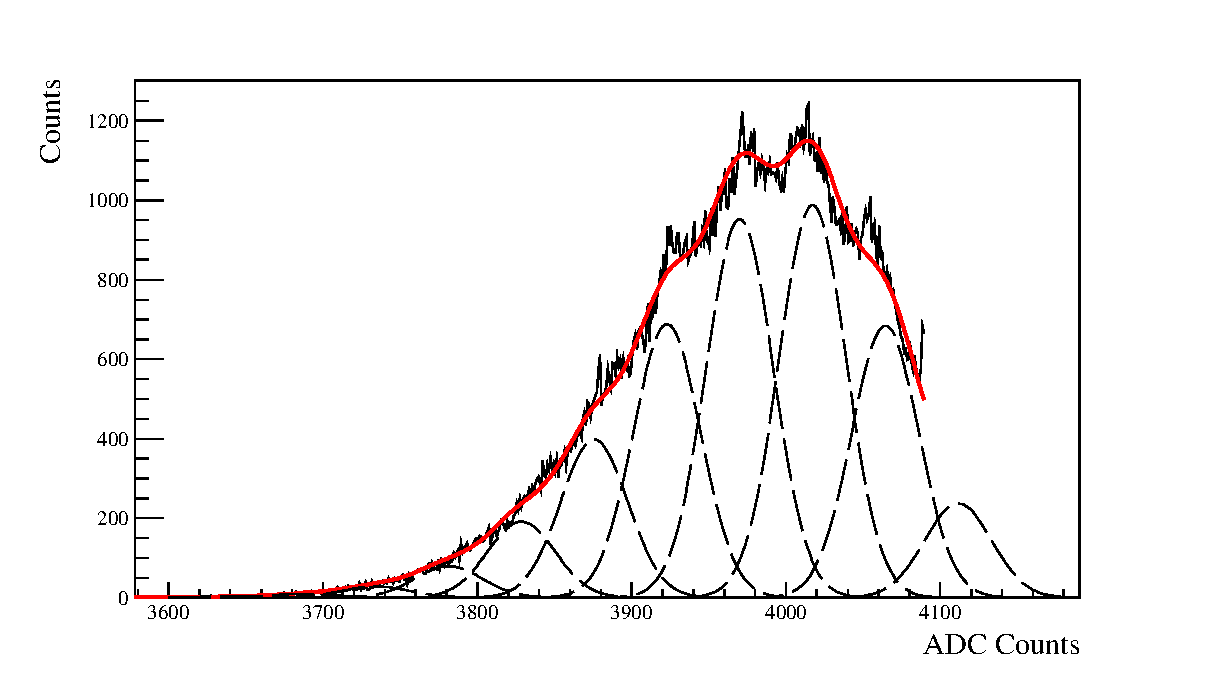
\includegraphics[width=1\textwidth]{dropout_example}
    \caption[Dropout Fit Example]{[black solid line] The measured baselines
    for run 101357 and [red] the best fit dropout model with the
    individual Gaussian distributions [black dashed line] that make up the best fit.}
\label{fig:dropoutexample}
\end{figure}


Figure~\ref{fig:dropoutexample} shows the measured dropout for run 101357.
The best fit extracts an average dropout of $\lambda=2.7$ channels.
For each run a similar dropout measurement is performed, the resulting dropout
rate is later used in simulation as part of the DAQ simulation.

\subsection{Nhit Monitor}
\label{sec:nhit_monitor}
During standard data taking a calibration, called the nhit monitor, is
performed to measure the effective threshold of the trigger N100 and N20
triggers.
The goal is to estimate the function $P_{\mathrm{trig}}(N)$,
called the trigger efficiency curve,
it's the probability of triggering at any given number of hits $N$.
The process for estimating that curve is to steadily increase the number of
PEDESTAL hits occurring at a single time and observe at which number of hits
the detector triggers, and how frequently it triggers.
For the entirety of the data taking only channels in
crate 4 of the detector were pedestalled for the nhit monitor.
This introduces the possibility of bias into the nhit monitor estimate
for the trigger efficiency curve.
Although all channels in the detector are designed to function identically, this
is not something that is closely monitored or tested, so it could be the case
that the channels on crate 4 are not representative of the detector as a whole.
For this reason the estimates of the trigger efficiency from the nhit monitor
are usually compared to other estimates from laserball data.

A value related to the number of hits in an event, called the ``in-time hits'' or
$\tilde{n}$,
is typically used for estimating the trigger efficiency.
The in-times hits is an estimate of the maximum height of the trigger pulse in
units of nhit, it includes effects from the pulse width of each trigger
and the average pulse rise-time.
Each event has two in-time nhit estimates one for the N100, $\tilde{n}_{100}$
and one for the N20, $\tilde{n}_{20}$.
Figure~\ref{fig:trigeff} shows the trigger efficiency from nhit monitor data
compared to data from simulation for the N100 trigger.
\begin{figure}[htbp]
    \centering
    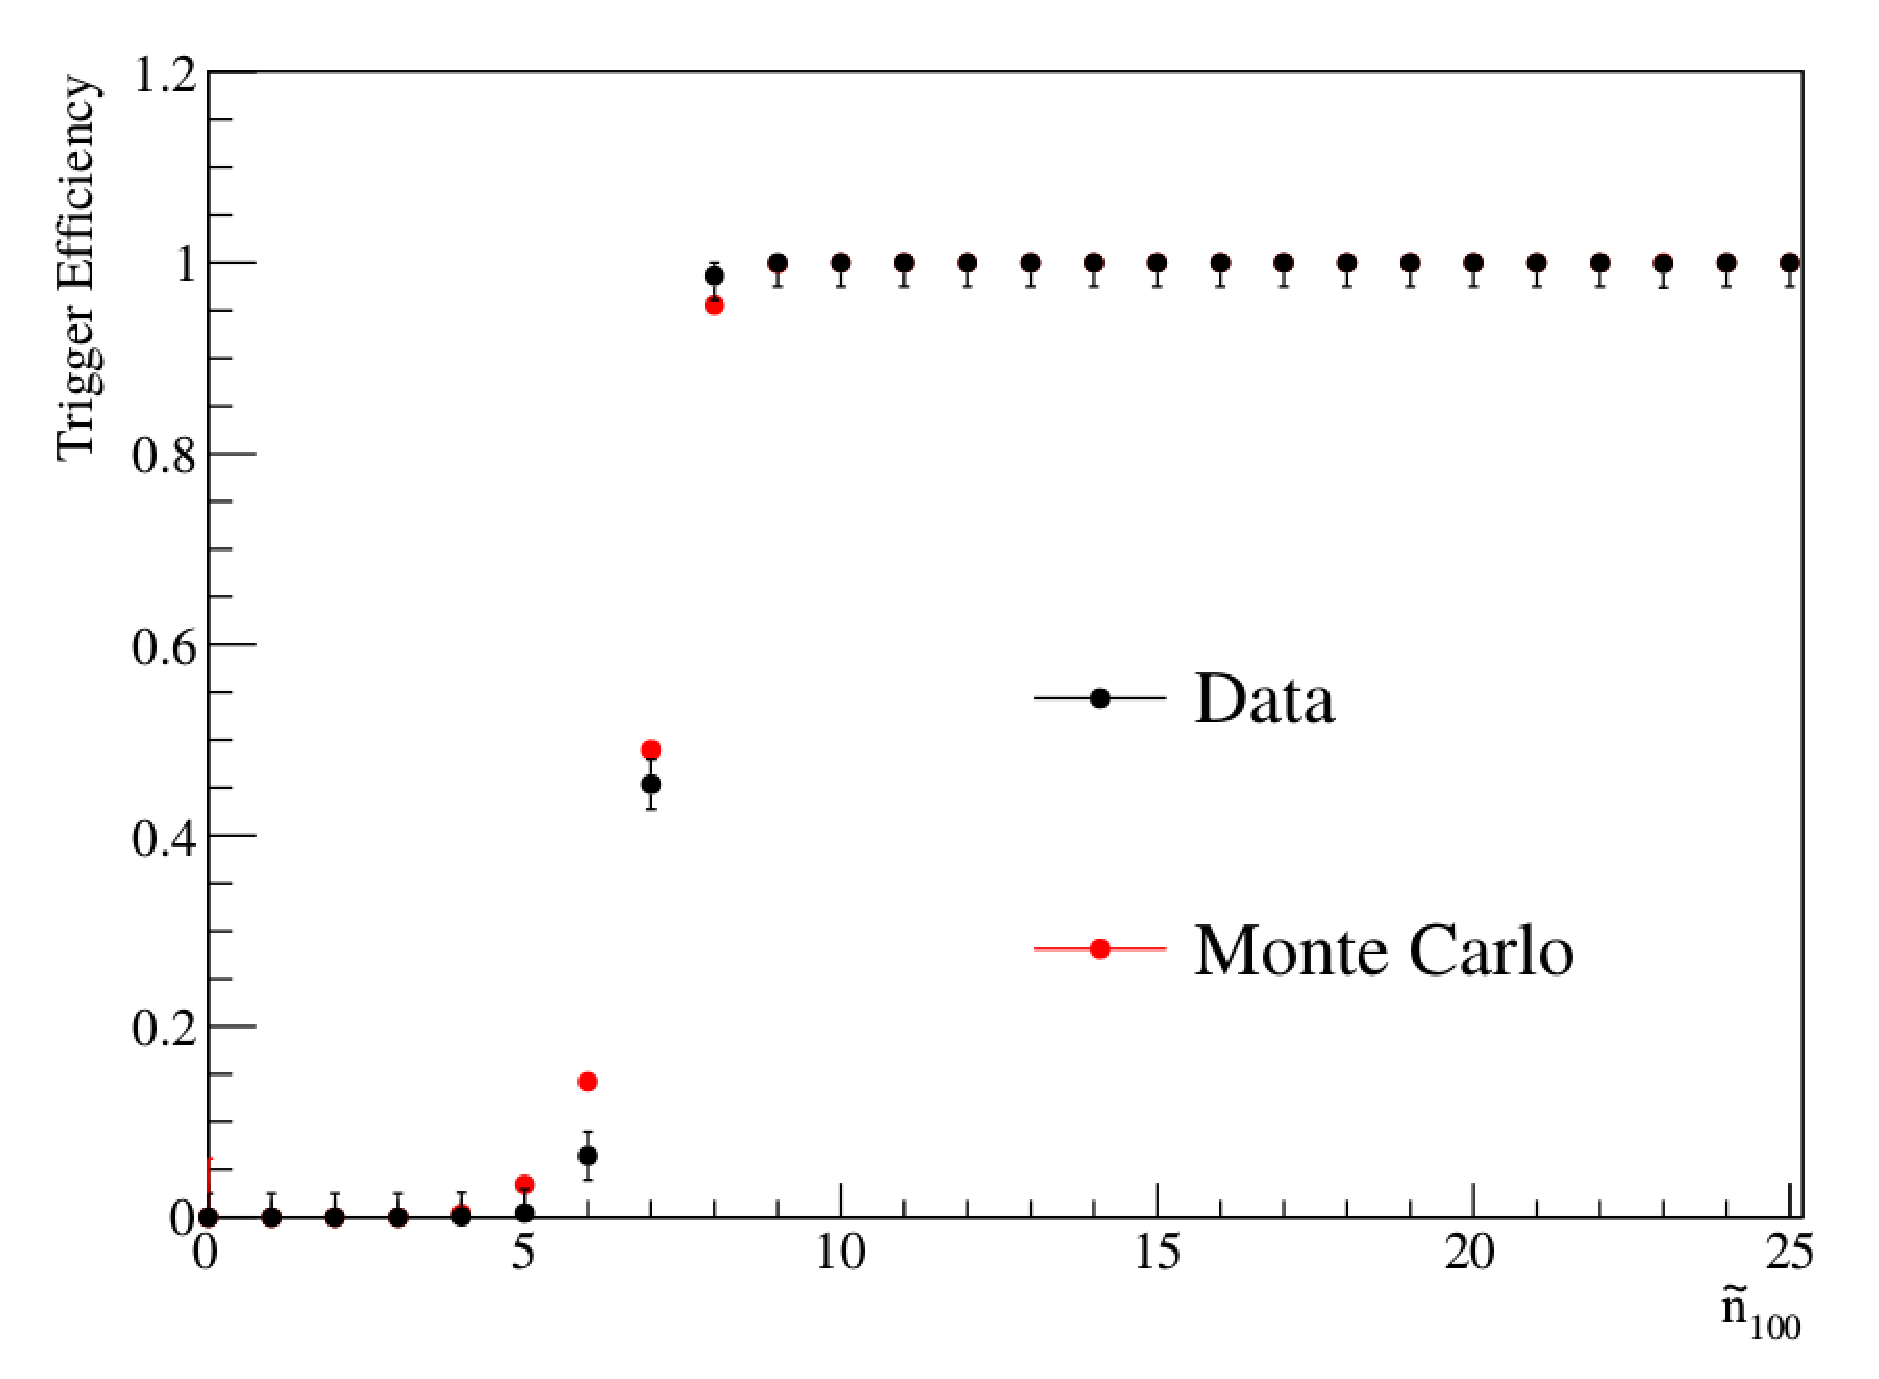
\includegraphics[width=0.73\textwidth]{trigger_efficiecy}
    \caption[Trigger Efficiency] {Comparison of the measured trigger efficiency
    and simulated trigger efficiency for run 107640. Plot from~\citep{tanner_triggeff}.}
\label{fig:trigeff}
\end{figure}

